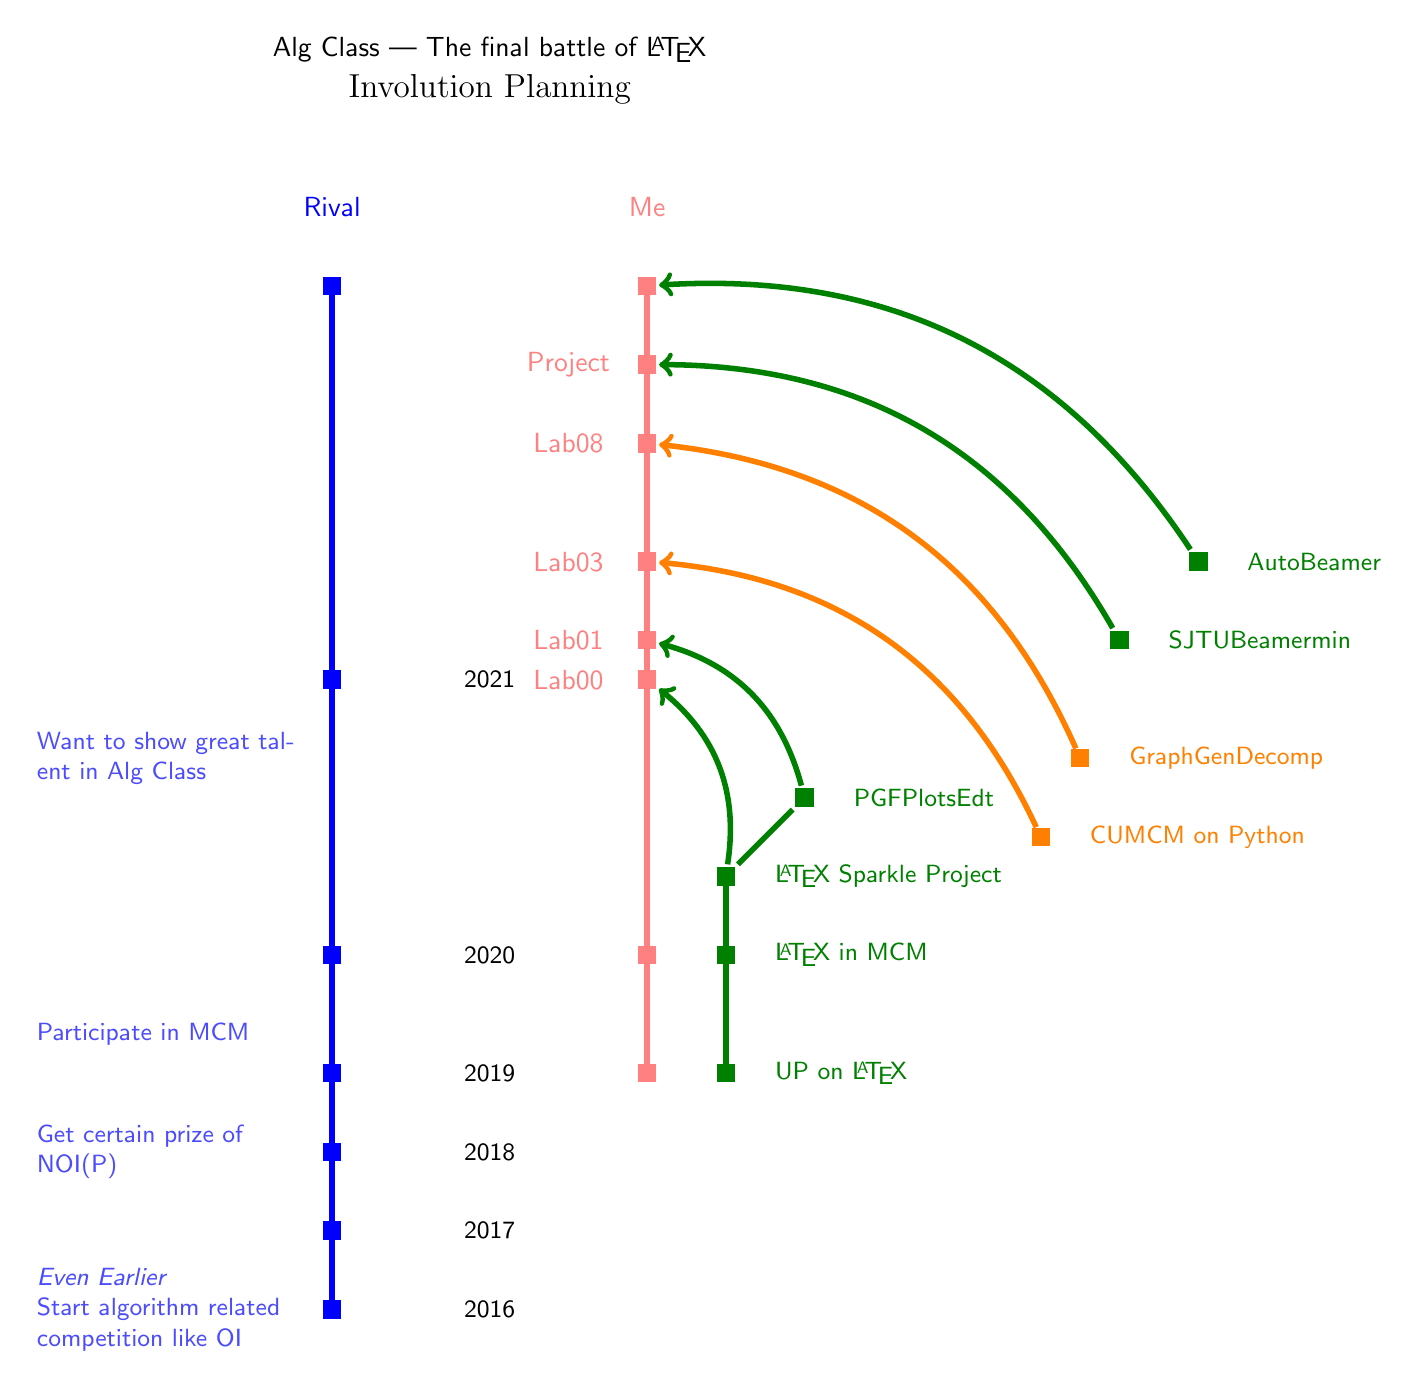
\begin{tikzpicture}
\tikzstyle{other} = [fill=blue];
\tikzstyle{otherline} = [blue,line width=2pt,font=\sffamily];
\tikzstyle{othercomment}=[text width=3.5cm,font=\sffamily\small,blue!70];
\tikzstyle{me} = [fill=red!50];
\tikzstyle{meline} = [red!50, line width=2pt, font=\sffamily];
\tikzstyle{mecomment} = [text width=3.5cm,font=\sffamily\small,red!70];
\tikzstyle{years} = [font=\sffamily\small];
\tikzstyle{branchn} = [above right,meline,text width=3.5cm];
\tikzstyle{branch} = [meline,bend left,->];
\tikzstyle{branchp} = [fill=green!50!black];
\tikzstyle{branchc} = [years,right,green!50!black];
\tikzstyle{branchline} = [green!50!black,line width=2pt];
\tikzstyle{branchsp} = [branchp,red!50!yellow];
\tikzstyle{branchsline} =[branchline,red!50!yellow,bend right,->];
\tikzstyle{branchsc} = [branchc,red!50!yellow];

\draw [otherline](-1,-7) node [other] {} -- (-1,-6) node [other] {} -- (-1,-5) node [other] {} -- (-1,-4) node [other] {} -- (-1,-2.5) node [other] {} -- (-1,1) node [other] {} -- (-1, 6) node [other] {};
\node [years] at (1,-7) {2016};
\node [years] at (1,-4) {2019};
\node [years] at (1,-2.5) {2020};
\node [years] at (1,1) {2021};
\node [otherline] at (-1,7) {Rival};
\node [otherline,black] at (1,9) {Alg Class --- The final battle of \LaTeX{}};
\node [font=\large] at (1,8.5) {Involution Planning};
\node [othercomment] at (-3,-7) {\emph{Even Earlier} \\Start algorithm related competition like OI};
\node [othercomment] at (-3,-5) {Get certain prize of NOI(P)};
\node [othercomment] at (-3,-3.5) {Participate in MCM};
\node [othercomment] at (-3,0) {Want to show great talent in Alg Class};
\draw [meline] (3,-4) node [me] {} -- (3,-2.5) node [me] {} -- (3,1) node [me] (v5) {} -- (3,1.5) node [me] (v2) {} -- (3,2.5) node [me] (v8) {} -- (3,4) node [me] (v9) {} -- (3,5) node [me] (v11) {} -- (3, 6) node [me] (v12) {};
\node [years] at (1,-6) {2017};
\node [years] at (1,-5) {2018};

\draw [branchline](4,-4) node [branchp] {} -- (4,-2.5) node [branchp] {} -- (4,-1.5) node [branchp] (v4) {} edge[bend right,->] (v5);
\node [branchc] at (4.5,-4) {UP on \LaTeX{}};
\node [branchc] at (4.5,-2.5) {\LaTeX{} in MCM};
\node [branchc] at (4.5,-1.5) {\LaTeX{} Sparkle Project};
\node [meline] at (2,1) {Lab00};
\node [meline] at (2,1.5) {Lab01};
\draw [branchline](5,-0.5) node [branchp] (v6) {} edge[bend right,->] (v2);
\draw [branchline] (v4) edge (v6);
\node [branchc] at (5.5,-0.5) {PGFPlotsEdt};
\node [meline] at (2,4) {Lab08};

\node [branchsp] (v7) at (8.5,0) {};
\node [branchsc] at (9,0) {GraphGenDecomp};
\node [branchsp] (v10) at (8,-1) {};

\node [branchsc] at (8.5,-1) {CUMCM on Python};
\node [meline] at (2,2.5) {Lab03};
\draw [branchsline] (v10) edge (v8);
\draw [branchsline] (v7) edge (v9);
\node [meline] at (2,5) {Project};
\draw [branchline](9,1.5) node [branchp] {} edge[bend right,->] (v11);
\node [branchc] at (9.5,1.5) {SJTUBeamermin};
\draw [branchline](10,2.5) node [branchp] {} edge[bend right,->]  (v12);
\node [branchc] at (10.5,2.5) {AutoBeamer};
\draw [branchline](v4);
\node [meline] at (3,7) {Me};
\end{tikzpicture}